\subsection{Теорема Штейнера. Доказательство. Примеры использования}

\begin{theorem}
    Теорема Штейнера.

    Если известен для тела момент инерции относительно оси, проходящей через центр тяжести, то момент инерции относительно оси параллельной ей определяется по формуле

    $$I=I_C+md^2$$

    где $I_0$ - момент инерции относительно оси, проходящей через центр тяжести
    $d$ - расстояние между осями
    $C$ - центр масс тела
\end{theorem}

\begin{figure}[h]
    \centering
    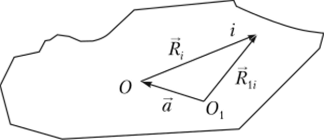
\includegraphics[width=0.5\linewidth]{imgs/q10i2.png}
\end{figure}

\begin{proof}
    Понять то, как меняется момент инерции при параллельном переносе оси, помогает теорема Штейнера. 
Рассмотрим произвольное твердое тело массы m в проекции, перпендикулярной оси вращения О, 
проходящей через центр масс тела. Рассмотрим другую произвольную ось вращения $O_1$ параллельную оси О 
и расположенную на расстоянии а от нее.

Момент инерции относительно оси О равен $J_0 = \sum\limits_{i=1}^\infty m_iR_i^2$.

Аналогично момент инерции относительно оси O, $J = \sum\limits_{i=1}^\infty m_iR_{1i}^2$

Воспользовавшись тем, что квадрат вектора равен квадрату его модуля и $\vec{R_{1i}}=\vec{R_i} + \vec{a}$, получим:

$$J 
= \sum\limits_{i=1}^\infty m_iR_{1i}^2 
= \sum\limits_{i=1}^\infty m_i(\vec{R_{i}} + \vec{a})^2
= \sum\limits_{i=1}^\infty m_i\vec{R_{i}}^2 + \sum\limits_{i=1}^\infty m_i\vec{a}^2 + 2\sum\limits_{i=1}^\infty m_i\vec{R_{i}}\vec{a} 
= 
$$
$$
= J_0 + \vec{a}^2\sum\limits_{i=1}^\infty m_i + 2\vec{a}\sum\limits_{i=1}^\infty m_i \vec{R_i}
$$

По определению центра масс последняя сумма равна нулю, откуда следует: 
$$J = J_0 + ma^2$$

Таким образом, доказана следующая теорема.

Теорема Штейнера: момент инерции тела относительно произвольной оси вращения равен сумме момента инерции этого тела, 
взятого относительно параллельной ей оси, проходящей через центр масс, и произведения массы тела на квадрат расстояния 
между осями.
\end{proof}

\begin{example}
    Примеры использования
\end{example}
\begin{figure}[h]
    \centering
    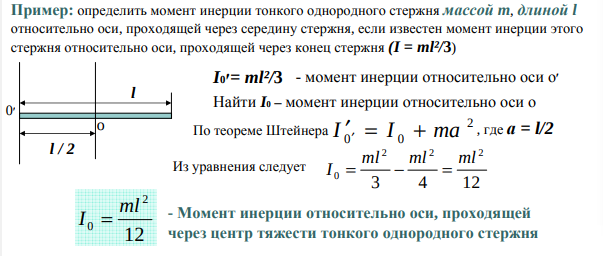
\includegraphics[width=0.7\linewidth]{imgs/q10i1.png}
\end{figure}
